\section{Enti normativi}
Il \textbf{CENELEC} è il comitato europeo di normazione elettrotecnica, in Italia invece l'ente normativo
è il \textbf{CEI}, Comitato Elettrotecnico Italiano che recepisce le normative europee e in genere le recepisce
traducendole senza apportare alcuna modifica, se il CEI ha invece già emanato una norma sull'argomento deve 
subito provvedere ad aggiornarla per renderla conforme con la normativa CENELEC, solitamente viene recepita
direttamente la norma CENELEC, ritirando quella italiana.

\textbf{Tipi di norme:}
\begin{itemize}
 \item \textbf{Base}: prettamente metodologica, descrizione della metodologia di prova, della strumentazione di misura
 con le sue caratteristiche, calibrazione dello stesso e ulteriori prescrizioni sui metodi di misura
 durante la validazione dell'elemento in prova. Non fissa alcun limite.
 \item \textbf{Generiche}: forniscono dei limiti e differenziano gli ambienti in cui i dispositivi vengono 
 utilizzati, ad esempio la suddivisione tra ambiente domestico, dove i dispositivi possono essere molto vicini
 tra loro, e l'ambiente industriale dove i dispositivi sono posti a distanze ragionevoli ed inoltre l'industria
 o l'azienda possiedono i fondi necessari alla ricerca di eventuali problemi di compatibilità.
 \item \textbf{Di prodotto}: fissano anch'esse dei limiti ma riguardano singoli prodotti o categorie di prodotti.
 Se per un prodotto non esiste una specifica norma, si applica la norma generica.
 \item \textbf{Armonizzate}: sono norme generiche o di prodotto, fatte proprie dall'unione europea e recepite,
 ``armonizzate'' dai vari stati includendole nel loro corpus normativo.
 \end{itemize}

Non sempre è necessario eseguire prove normate, ci si può affidare ad organismi terzi per verificare
il soddisfacimento dei requisiti. È possibile inoltre dimostrare la compatibilità elettromagnetica del proprio
prodotto utilizzando unicamente il progetto, se questo è in grado di dimostrare intrinsecamente il 
soddisfacimento dei requisiti imposti. È comunque preferito molto spesso l'approccio sperimentale per
la difficoltà molto spesso di avere un modello che copra tutti i range di frequenze.

Il CENELEC fu fondato nel '73 e composto dai comitati tecnici dei singoli paesi europei, inclusi affiliati
esterni che partecipano alle discussioni ma senza diritto di voto, è finalizzato all'armonizzazione: raccoglie 
ed elabora le norme emesse da altri enti (es. IEC) al fine di garantire uno standard richiesto dal mercato
europeo.

L'origine di una norma si riconosce mediante la sua sigla, ad esempio EN 50157-2-1.
\newpage
Le normative europee sono così numerate:
\begin{itemize}
 \item \textbf{40000/44999} derivano da una standardizzazione congiunta del CEN e del CENELEC riguardo
 il settore IT.
 \item \textbf{45000/49999} riguardano le attività congiunte CEN e CENELEC al di fuori del settore IT.
 \item \textbf{50000/59999} riguardano le attività esclusive del CENELEC.
 \item \textbf{60000/69999} l'implementazione da parte del CENELEC delle norme IEC.
\end{itemize}
Ad esempio la normativa europea EN 61000-4-3 deriva dalla IEC 1000-4-3 con le eventuali modifiche, la 
norma CISPR-16 è stata recepita in Europa con il numero EN 55016. 

\section{Approccio al problema}
Come ci si approccia al problema della compatibilità? Esiste l'approccio di \textbf{crisi}: si tenta di risolvere il
problema di compatibilità solo in fase di collaudo finale, senza tenere precedentemente in considerazione
eventuali problemi.
Questo approccio è molto rischioso dato che eventuali costi connessi alla soluzione saranno molto elevati
a causa della necessità di agire su un prodotto finito.

L'alternativa è l'approccio \textbf{sistematico}, ossia la considerazione dei problemi di compatibilità sin dalle fasi iniziali
della progettazione del prodotto, in questo modo è possibile risparmiare sui costi agendo in maniera tempestiva
su eventuali problemi e senza dover ritardare il rilascio del prodotto sul mercato.
Eventuali soluzioni potrebbero essere lo spostamento di una pista o l'allontanamento di due parti sensibili,
tutte queste procedure, in fase di progetto, sono economiche da applicare.
Questa tipologia di approccio prevede inoltre l'esecuzione di molteplici verifiche intermedie, a partire
da soluzioni simulate con un modello matematico fino a prove dirette sui prototipi iniziali.
\begin{figure}[h]
 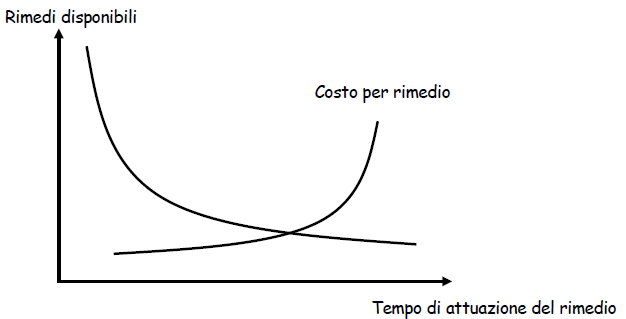
\includegraphics[width=0.7\linewidth]{costo_rimedio.png}
 \centering
 \caption{Rappresentazione del costo per rimedio in funzione del tempo di attuazione}
 \label{fig:costo_rimedio}
\end{figure}
%\newpage
Se il sistema è complesso si può dividere la scheda in più sezioni e analizzare le singole parti,
semplificando le analisi.

Gli ``attori'' che partecipano al fenomeno della compatibilità elettromagnetica sono sicuramente
almeno due: la \textbf{sorgente} e la \textbf{vittima}, tra i due è interposto il canale di accoppiamento.
Il disturbo può colpire la vittima mediante varie \textit{porte} come le porte di comunicazione,
di alimentazione o la porta ``involucro''.

I \textit{canali di accoppiamento} sono le vie utilizzate dai disturbi o dai segnali utili per propagarsi tra i 
dispositivi, il cavo di alimentazione può trasmettere disturbi al dispositivo provenienti dalla rete di alimentazione
ma può essere comunque protetto con un filtro, il discorso si complica per i canali di accoppiamento non previsti,
ovvero canali che non dovrebbero trasmettere alcuna informazione o energia utile per l'apparecchio.

\begin{figure}[h]
 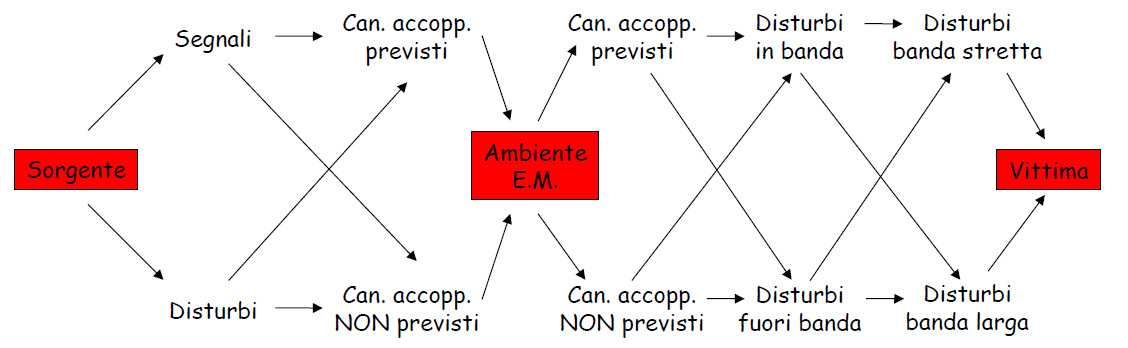
\includegraphics[width=0.7\linewidth]{catena_disturbi.png}
 \centering
 \caption{Rappresentazione della catena dei canali di accoppiamento dei disturbi}
 \label{fig:catena_disturbi}
\end{figure}

I disturbi che si propagano nella vittima possono rientrare o meno nella sua \textbf{banda} di funzionamento
ossia l'intervallo di frequenze alle quali è previsto il funzionamento del dispositivo, un disturbo si dice
a \textit{banda stretta} se rientra nella banda di funzionamento del dispositivo, si dice a \textit{banda larga}
se la sua ampiezza supera la banda di funzionamento del dispositivo.
Un disturbo a banda stretta (\textit{NarrowBand}) probabilmente potrà accoppiarsi con il dispositivo mediante
canali di accoppiamento previsti e risultare udibile per l'utente (ad esempio nel caso di un disturbo radiato che colpisce
un ricevitore FM).
Un disturbo a banda larga (\textit{BroadBand}) non rientra nelle caratteristiche di funzionamento del dispositivo
e potrà utilizzare con buona probabilità anche canali non previsti.
Un segnale composto da una singola componente in frequenza è un segnale a banda stretta per antonomasia.
\begin{figure}[h]
 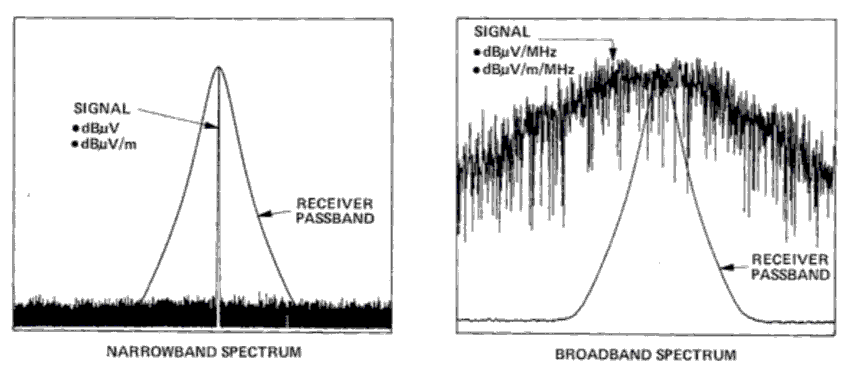
\includegraphics[width=0.7\linewidth]{narrow-broadband.png}
 \centering
 \caption{Confronto tra segnali a banda stretta e larga rispetto al filtro di un ricevitore}
 \label{fig:narrow-broadband}
\end{figure}






